\chapter{Optimisation of Experimental Parameters}
\label{chap:experimental_optimisation}

The previous chapter considered intrinsic platform properties that are fixed once the system has been fabricated or purchased. This chapter instead examines experimentally adjustable parameters that can be modified during operation. The influence of the optical beam dimensions, beam geometry, and magnetic-field homogeneity is evaluated through their effect on the fibre-coupled retrieval.

\section{Optical Beam Geometry}
\label{sec:results_optical_beam_geometry}

The optical geometry determines both the spatial extent of the prepared spin wave and the phase-matching conditions for retrieval. The beam widths and relative propagation directions are therefore considered separately.

\subsection{Beam Width}
\label{sec:results_beam_width}

The signal and control fields are represented by Gaussian transverse profiles whose diameters can be modified through the optical focusing system. Changing the beam widths alters the number of atoms contributing significantly to the prepared and retrieved modes, as well as the distance that an atom must travel before its optical weight becomes small.

A wider interaction region reduces the sensitivity to transverse atomic motion. In the warm-vapour system, diffusing atoms must travel farther before leaving the region of significant mode overlap. In the cold-atom system, a larger mode similarly increases the ballistic transit time across the illuminated region. For fixed atomic preparation and transport parameters, increasing the beam width is therefore expected to extend the decay time of the fibre-coupled retrieval.

The comparison between the warm-vapour and cold-atom systems is shown in Fig.~\ref{fig:beam_width_scan}. Although the transport mechanisms differ, the same geometric effect is observed in both platforms. Larger optical modes remain overlapped with the moving ensemble for longer times and consequently produce a slower reduction of the retrieved signal.

\begin{figure}[htbp]
    \centering
        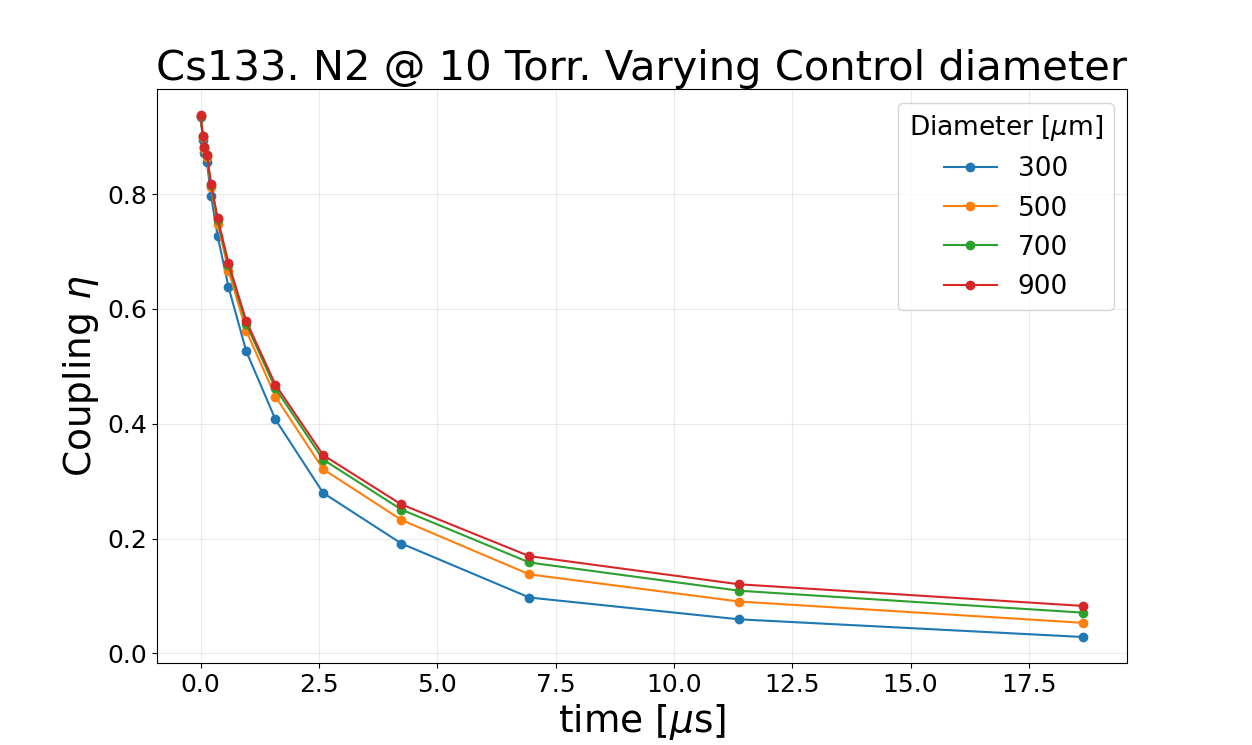
\includegraphics[width=0.78\textwidth]{Figures/beam_size_scan_coupling_decay.jpeg}
    \caption{Normalized fibre-coupled retrieval for different magnetic-field gradients. A spatially varying ground-state splitting causes different parts of the ensemble to accumulate different phases, thereby reducing constructive retrieval into the target optical mode.}
    \label{fig:magnetic_gradient_scan}
\end{figure}



\subsection{Control--Signal Beam Angle}
\label{sec:results_beam_angle}

A non-zero angle between the signal and control beams can assist the spatial separation and filtering of the weak retrieved signal from the strong control field. This experimental advantage is accompanied by a change in the spin-wave wave vector,
\begin{equation}
    \Delta\mathbf{k}
    =
    \mathbf{k}_{\mathrm{sig}}
    -
    \mathbf{k}_{\mathrm{ctrl}}.
\end{equation}
Increasing the angle increases $|\Delta\mathbf{k}|$ and reduces the corresponding spin-wave wavelength. Atomic motion then produces a larger phase change for a given displacement,
\begin{equation}
    \delta\phi_j(t)
    =
    \Delta\mathbf{k}\cdot
    \left[
        \mathbf{r}_j(t)-\mathbf{r}_j(0)
    \right].
\end{equation}

The collective readout therefore becomes more sensitive to atomic motion as the angle is increased. The beam angle must consequently be selected by balancing the improved spatial filtering against the resulting increase in motion-induced spin-wave dephasing.
\section{Magnetic-Field Homogeneity}
\label{sec:results_magnetic_gradient}

In addition to motion-induced loss of spatial overlap, collective retrieval can be reduced by magnetic-field inhomogeneity. The relevant quantity is the differential Zeeman shift of the two ground states forming the stored coherence,
\begin{equation}
\Delta\omega_{sg}(B)
=
\frac{E_s(B)-E_g(B)}{\hbar}.
\end{equation}
For sufficiently weak fields, this shift can be approximated as
\begin{equation}
\Delta\omega_{sg}(B)
\simeq
\Delta\omega_{sg}^{(0)}
+
\beta B,
\qquad
\beta
=
\frac{\mu_{\mathrm B}}{\hbar}
\left(
g_{F_s}m_{F_s}
-
g_{F_g}m_{F_g}
\right),
\label{eq:results_zeeman_sensitivity}
\end{equation}
where $\beta$ denotes the differential magnetic sensitivity of the selected ground-state coherence. A spatially uniform magnetic field produces the same phase shift for all atoms. For a single selected coherence, this common phase changes the phase of the retrieved optical field but does not reduce its intensity. Dephasing is produced only by spatial variations of the field, since different atoms then accumulate different phases before retrieval.

The origin and structure of these inhomogeneities differ between the two platforms. In a warm-vapour cell, external magnetic fields can be strongly attenuated by $\mu$-metal shielding, although residual gradients may remain because of shield apertures, remanent magnetization, nearby magnetic materials, heater currents, and imperfect compensation. Laboratory measurements indicate residual gradients of order $\SI{10}{\nano\tesla\per\centi\metre}$. In a cold-atom experiment, the quadrupole field used for the magneto-optical trap must be switched off before the memory sequence. The residual field is then determined by coil-current decay, eddy-current transients, compensation errors, and spatial curvature. Its evolution can be both time dependent and non-linear across the expanding cloud, which makes a realistic field model strongly dependent on the specific coil geometry, switching electronics, and surrounding conducting structures. The smaller initial size of the cold ensemble reduces the field variation sampled at short times, but ballistic expansion increases the sampled volume during longer storage intervals and may expose higher-order spatial variations. Because these details are experiment specific and are not constrained by the present model, the numerical study is restricted to a static linear magnetic-field gradient in the warm-vapour system. This simpler case isolates the basic phase-scrambling mechanism and allows the required field homogeneity to be assessed without introducing poorly determined cold-atom transients.
The magnetic phase accumulated by atom $j$ is calculated along its trajectory as
\begin{equation}
\delta\phi_j(t)
=
\int_0^t
\left[
\Delta\omega_{sg}
\left(
\mathbf r_j(t')
\right)
-
\Delta\omega_{\mathrm{ref}}
\right]
dt',
\label{eq:results_magnetic_phase}
\end{equation}
where $\Delta\omega_{\mathrm{ref}}$ removes the common frequency shift. In the present simulation, the magnetic field is approximated by a linear axial gradient,
\begin{equation}
B_z(z)
=
B_0+G_z z,
\qquad
G_z
=
\frac{\partial B_z}{\partial z}.
\label{eq:results_linear_magnetic_gradient}
\end{equation}
The corresponding relative phase is therefore
\begin{equation}
\delta\phi_j(t)
=
\beta G_z
\int_0^t
\left[
z_j(t')-z_{\mathrm{ref}}
\right]
dt'.
\label{eq:results_linear_gradient_phase}
\end{equation}
This model assumes a fixed quantization axis and isolates dephasing caused by the longitudinal field component. Transverse-field-induced state mixing and time-dependent magnetic noise are not included.
The magnetic-gradient scan is performed for a warm $^{133}\mathrm{Cs}$ ensemble contained in a cylindrical cell of length $\SI{75}{\milli\metre}$ and diameter $\SI{4}{\milli\metre}$. The cell contains $\SI{10}{\Torr}$ of $\mathrm{N_2}$ buffer gas and is operated at $\SI{75}{\degreeCelsius}$. The signal and control beams have FWHM diameters of $\SI{120}{\micro\metre}$ and $\SI{300}{\micro\metre}$, respectively. The stored coherence is formed between
\begin{equation}
    \ket{g}
    =
    \ket{F=3,m_F=+3},
    \qquad
    \ket{s}
    =
    \ket{F=4,m_F=+4}.
\end{equation}
This coherence is linearly sensitive to magnetic fields, with a weak-field sensitivity of approximately
    $\frac{\beta}{2\pi}
    \simeq
    \SI{2.45}{\hertz\per\nano\tesla}.
$
Axial gradients between $\SI{0}{\nano\tesla\per\centi\metre}$ and $\SI{1e3}{\nano\tesla\per\centi\metre}$ are applied along the propagation direction. Since the cell is considerably longer than it is wide, an axial gradient produces the largest field variation across the ensemble for a given gradient magnitude and therefore provides a conservative test case.

\begin{figure}[htbp]
    \centering
    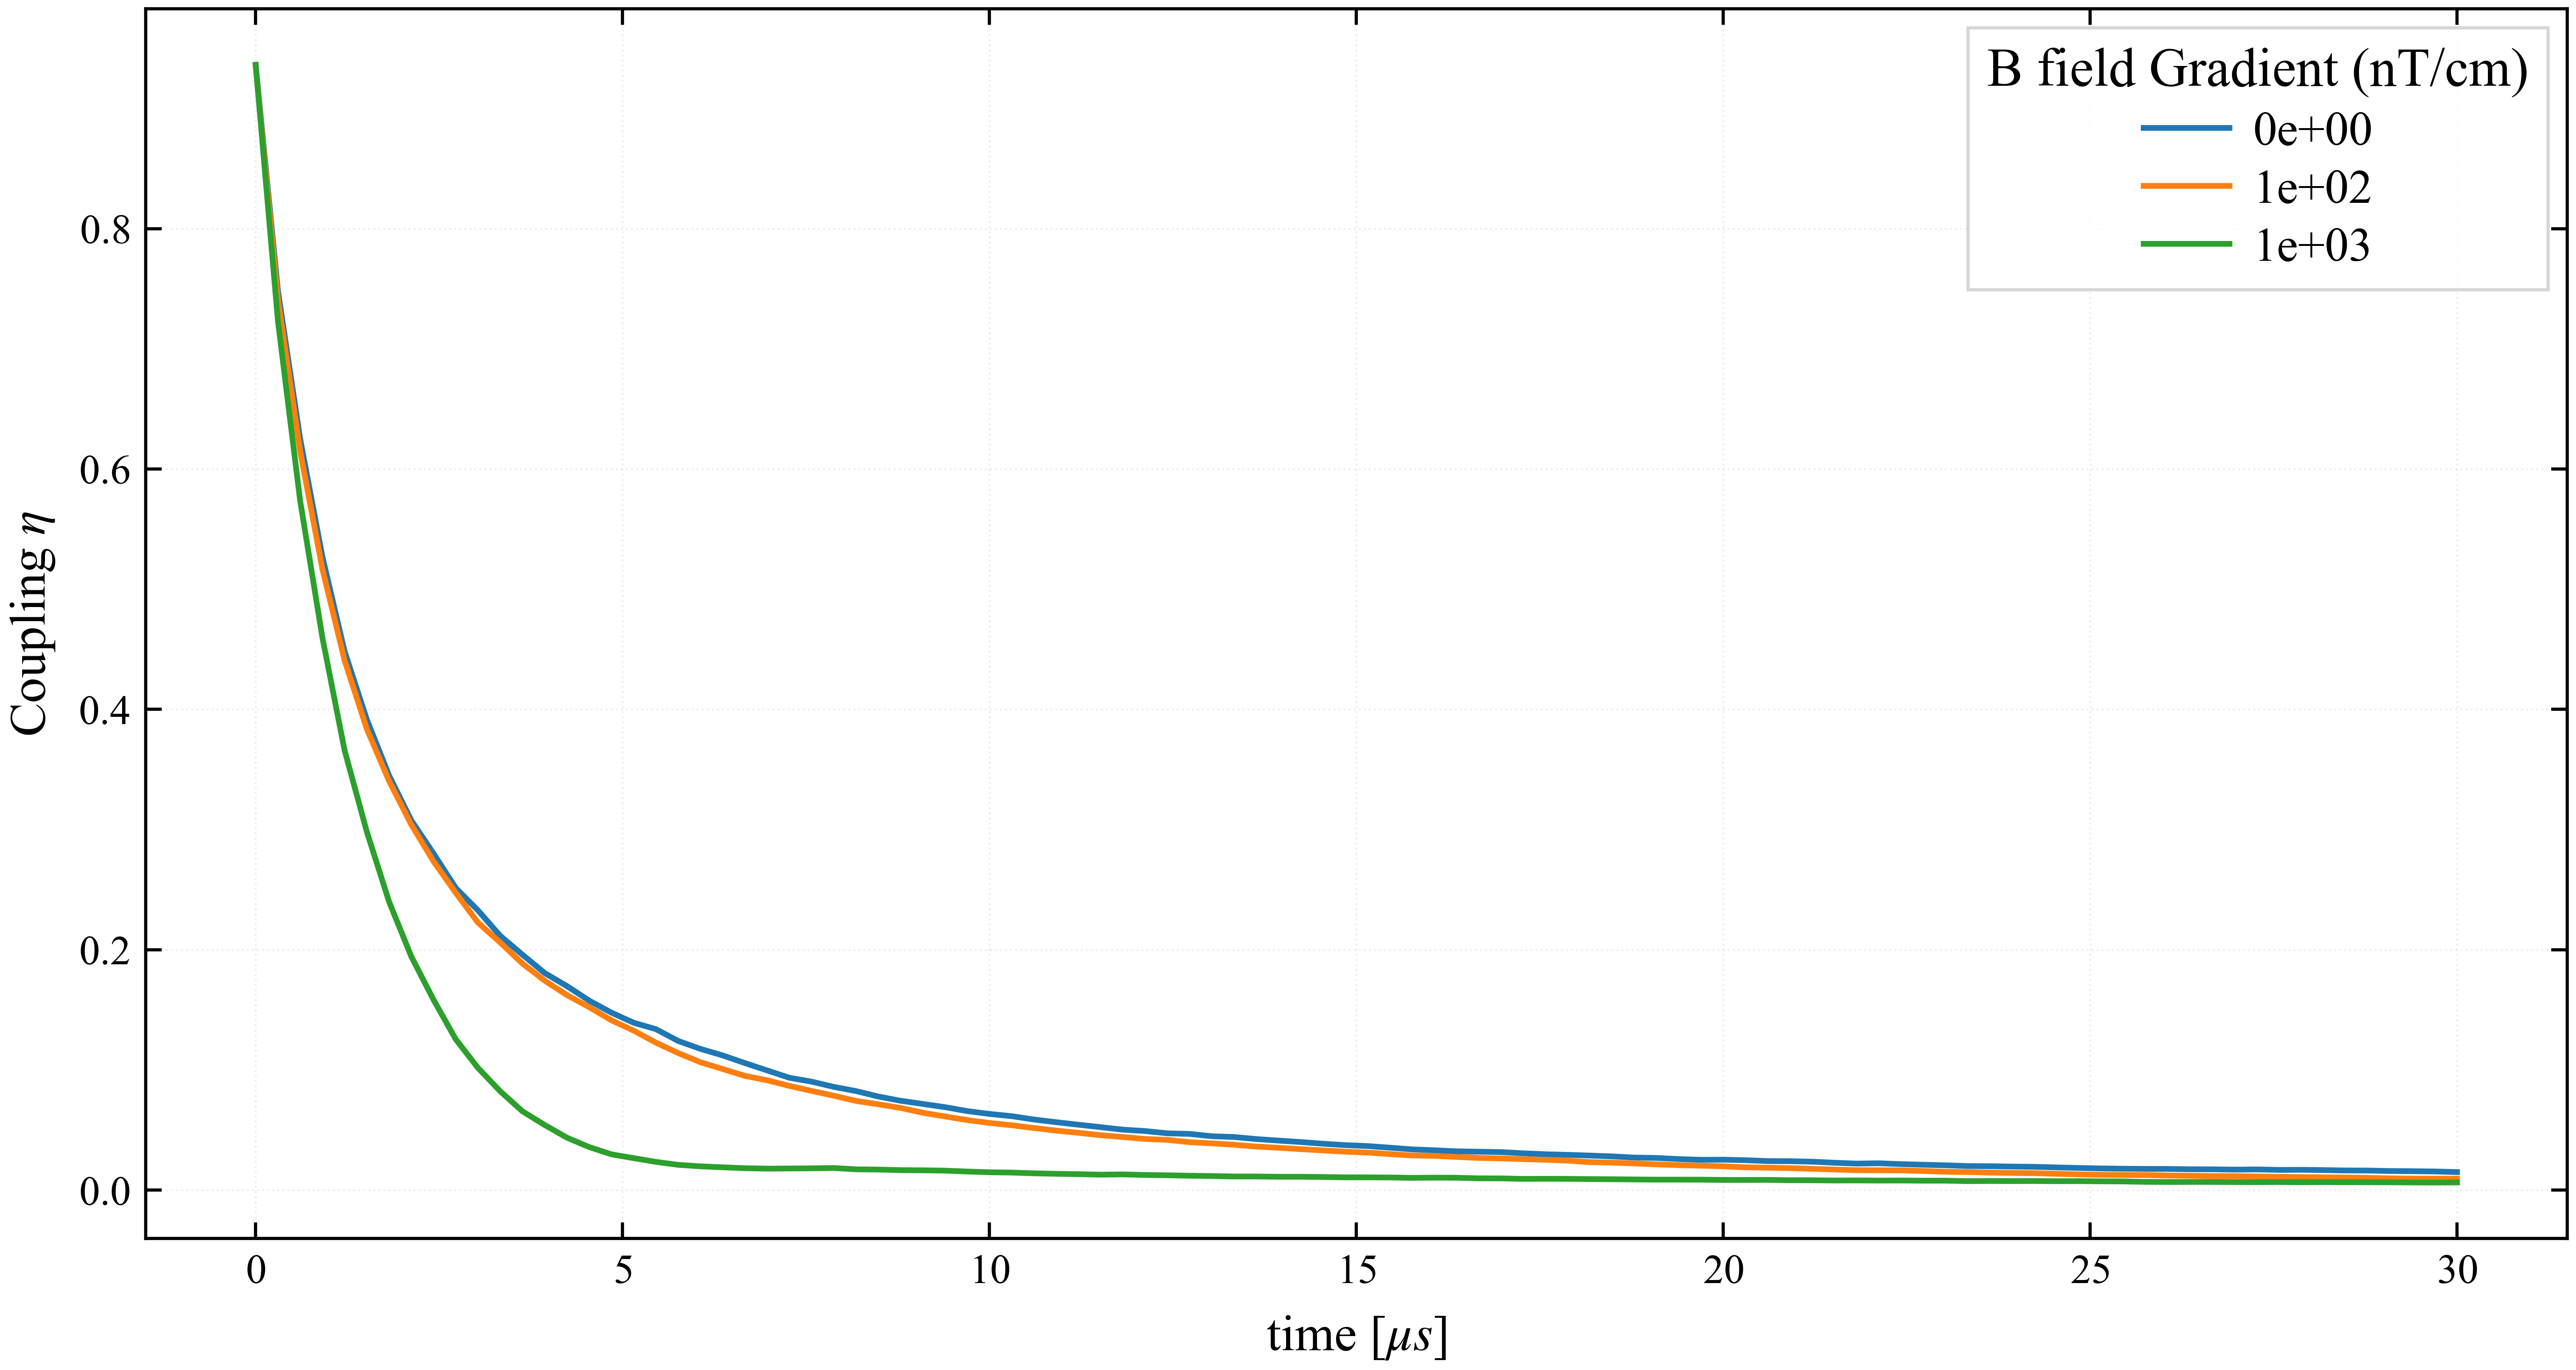
\includegraphics[width=0.72\textwidth]{Figures/magnetic_gradient_scan.png}
    \caption{Normalized fibre-coupled retrieval for different axial magnetic-field gradients $G_z=\partial B_z/\partial z$. The simulation considers a $^{133}\mathrm{Cs}$ cell of length $\SI{75}{\milli\metre}$ and diameter $\SI{4}{\milli\metre}$, operated at $\SI{75}{\degreeCelsius}$ with $\SI{10}{\Torr}$ of $\mathrm{N_2}$ buffer gas. The signal and control beams have FWHM diameters of $\SI{120}{\micro\metre}$ and $\SI{300}{\micro\metre}$, respectively.}
    \label{fig:magnetic_gradient_scan}
\end{figure}

Figure~\ref{fig:magnetic_gradient_scan} shows that the simulated retrieval remains close to the zero-gradient result for gradients up to approximately $\SI{1e2}{\nano\tesla\per\centi\metre}$ over the considered time interval. At larger gradients, the accumulated phase spread becomes appreciable and the fibre-coupled retrieval decays more rapidly. The gradient tolerance depends on the magnetic sensitivity of the selected coherence, the ensemble dimensions, the atomic trajectories, and the retrieval time.

The onset of magnetic dephasing in the simulation occurs at gradients approximately three orders of magnitude larger than those measured in the laboratory. Under the present warm-vapour conditions, magnetic-field inhomogeneity is therefore not expected to be the dominant limitation on the retrieved mode. Nevertheless, magnetic shielding and active field compensation remain necessary because this dephasing mechanism cannot be mitigated by increasing the optical beam size. An atom may remain within the illuminated region while ceasing to contribute constructively once its internal phase is no longer aligned with the remainder of the ensemble. Magnetic homogeneity must therefore be controlled independently of the spatial-overlap losses considered in the preceding sections.
